\documentclass{article}
\usepackage{graphicx} % Required for inserting images
\usepackage{float}


\title{24.05.07 Cardano Bridge}
\author{Xun Zhang \quad \quad Bingsheng Zhang \\ 
Zhejiang University, CHN \\
22221024@zju.edu.cn \quad bingsheng@zju.edu.cn}

\date{May 07 2024}
\begin{document}

\maketitle

\section{Background}

\textbf{Q: What is a Bridge?}

\noindent\textbf{Answer:}A bridge is a two way communication protocol that proves the occurrence of events in one chain C1 to applications in another chain C2 and vice-versa. For simplicity we use the terminology, \textbf{origin chain }(C1) and \textbf{target chain} (C2), though it is interchangeable.


The transmission of information between chains can be:
\begin{itemize}
    \item messages
    \item funds
    \item other data
\end{itemize}

The state change on the C1 has to be verified \textbf{“on-chain”} on C2. This is typically done by a \textbf{lightweight client}: a contract on the C2 that keeps track of a set of block headers on C1, and verifies them with a Merkle Proof corresponding to a root submitted from the origin chain. 
\\

\noindent\textbf{Q:Why we need a zero knowledge bridge?}

\noindent\textbf{Answer:}In general, C1 and C2 could operate in different domains, and verification operations require out of field arithmetic. Besides the list of headers continuing to increase, the client would require the storage and verification of new headers as they come along. This leads to significant computational and storage overheads, and is in general inefficient. To bypass this problem, many bridge constructions have taken a more centralized approach:

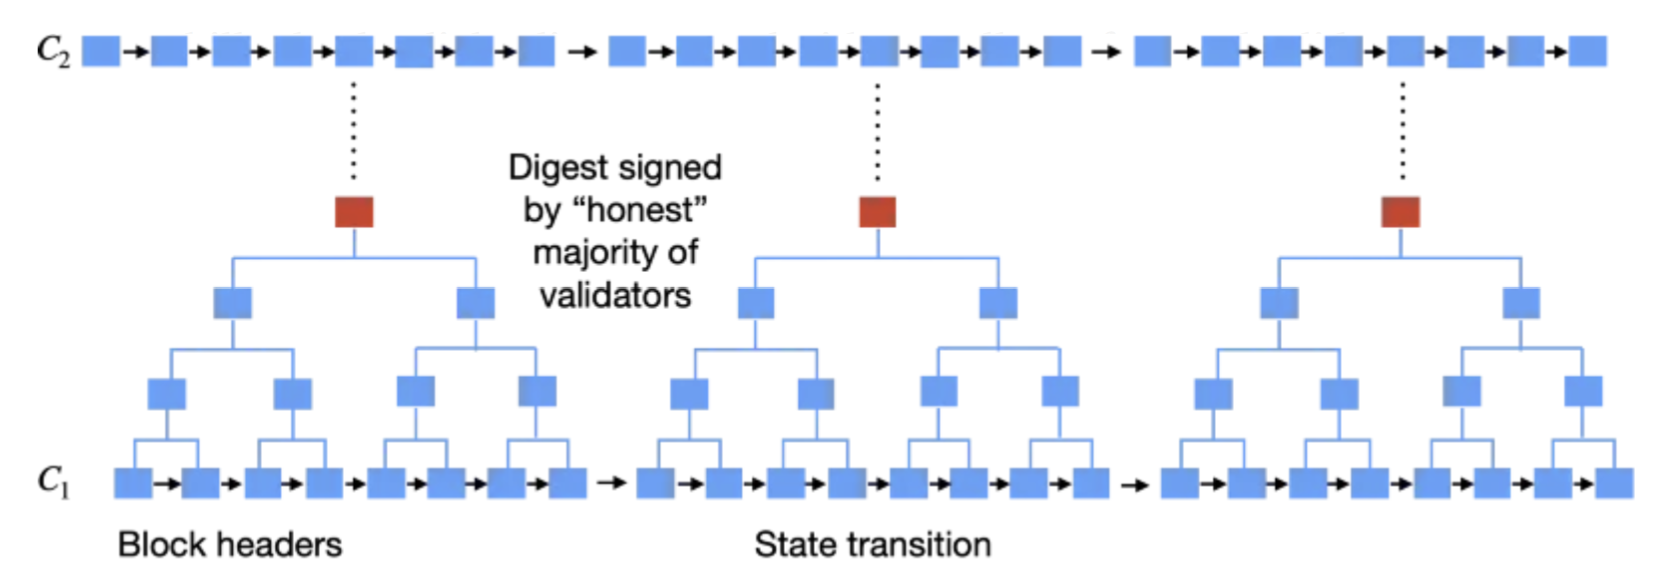
\includegraphics[width=1\linewidth]{2024-05-01 144803.png}
This is typically in the case of transfer of funds where substantial trust assumptions are placed on the centralized bridging entity, which usually consists of a small number of trusted parties. Notwithstanding the fact that this goes against the very founding principles of blockchains, it brings with it issues related to censorship and security.

Overall, the main technical challenge in building a bridge lies in:
\begin{itemize}
    \item Low computational overhead (efficiently handling cross domain data, out of field arithmetic).
    \item Low storage overhead. (Succinctness)
    \item Security/trustless (Soundness)
\end{itemize}


We choose zero knowledge proofs to overcome these problems.


\section{Existing Zero Knowledge Bridges}

There are three typical zero knowledge bridges:

\begin{itemize}
    \item Succinct by Succinct Labs: bridging from \textbf{Ethereum 2.0 }to \textbf{Gnosis}.
    \item ZKIBC by Electron Labs: bridging from \textbf{Cosmos SDK(Tendermint)} to \textbf{Ethereum}.
    \item zkbridge by Berkley RDI: bridging from \textbf{Cosmos SDK(Tendermint)} to \textbf{Ethereum}.
\end{itemize}

Below we provide a quick comparison of the various features of the three bridges:

\begin{table}[H]
    \centering
    \begin{tabular}{p{2cm}p{4cm}p{4cm}p{4cm}} \hline 
                        & Succinct labs & zkIBC &  zkBridge\\ \hline
         Verification Task   
         & Sync Committee: 512 high stake signatures

         Verification of Ethereum BLS signatures on Gnosis
         &  Verification of EdDSA Curve25519 signatures on Ethereum
         
         Validators: 32 high stake signatures
         & Verification of EdDSA Curve25519 signatures on Ethereum
         
         Validators: 32 high stake signatures
         

         \\ \hline
          Zk-proofs & Groth16 &Groth16 & deVirgo+Groth16 \\ \hline

         Constraint Size & 
         Sync Committee rotation: 68M constraints

         Verify signed header: 21M constraints
         &
         2.5M constraints for every Ed25519 signature
         
         & 2.5M constraints for every Ed25519 signature\\ \hline

      
    \end{tabular}
    \caption{Comparison of three bridges}
    \label{tab:my_label}
\end{table}


\section{Architecture}

We plan to use the architecture in zkbridge:

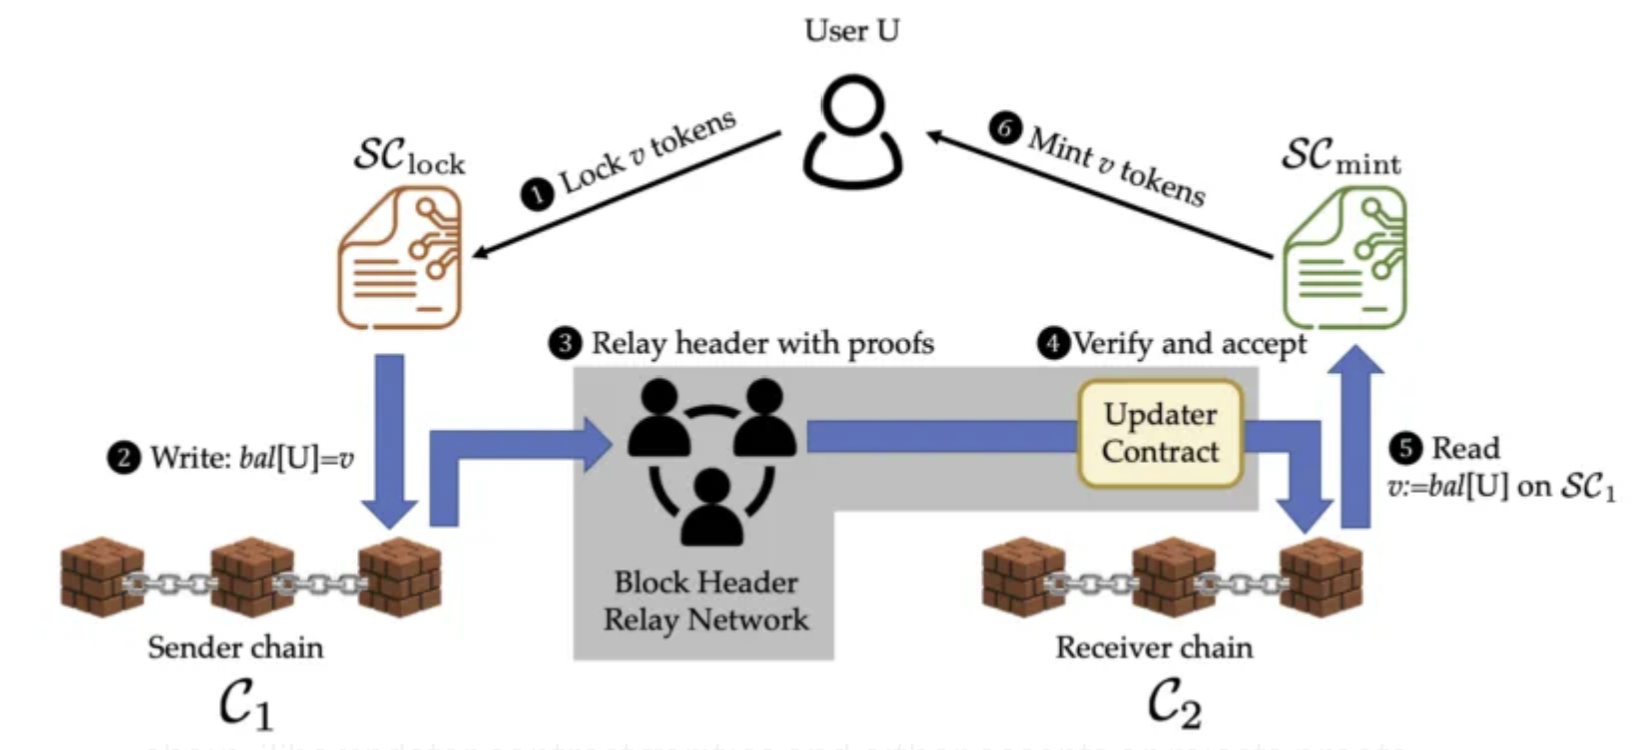
\includegraphics[width=1\linewidth]{2024-05-01 153459.png}

The block header relay network consists of a network of relay nodes that listen to the state changes on the bridged chains, and retrieve block headers from the full nodes in the blocks. The main functionality of a relay node on the bridge is to generate a ZKP that attests to the correctness of the block headers from one chain and relays it to the updater contract on the other chain. The updater contract verifies and either accepts or rejects proofs from nodes in the relay network.

The following figure shows a similar architecture of the bridge oevr Cardano:


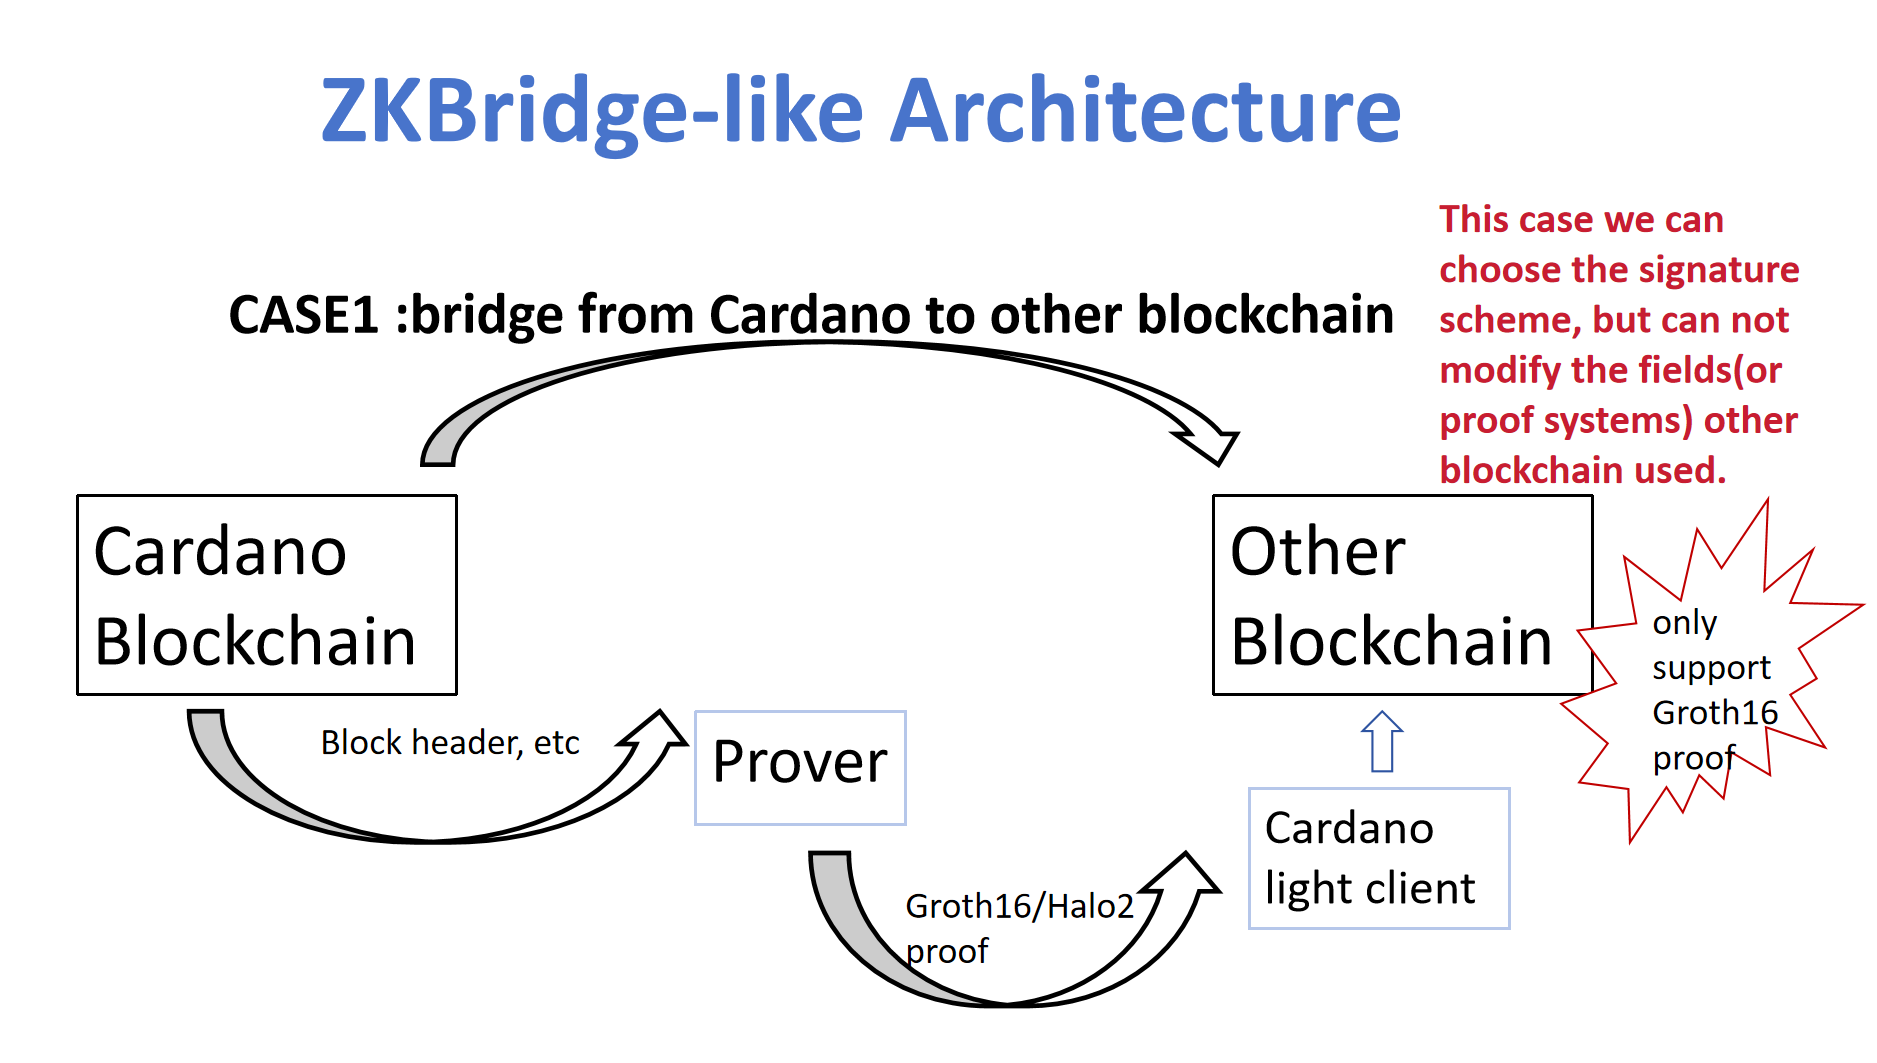
\includegraphics[width=1\linewidth]{cardano_bridge.png}


\section{Signature Scheme}

Since we want to construct a bridge between Cardano and other blockchains, the first thing we should consider is the verification task in our construction. That is, what things does our proof system need to prove.

Similar to ZKIBC and zkBridge, the main task of our bridge is to prove the state update over Cardano blockchain. Of which the most important part is to prove the correctness of signature. 




We consider combing the zero knowledge proofs with signature scheme. 
Imagine a sufficiently simple (but not practical) scenario: using Halo2/Groth16 to prove the correctness of aggregation and straightly verify BLS signature. Taking \textbf{Mithril} as an example, we can use zk-snark to prove the aggregation phase in signing process, and the verifier can verify the aggregated signature straightly. The following figure shows the simplified process of \textbf{Mithril} protocol:
\\
\\



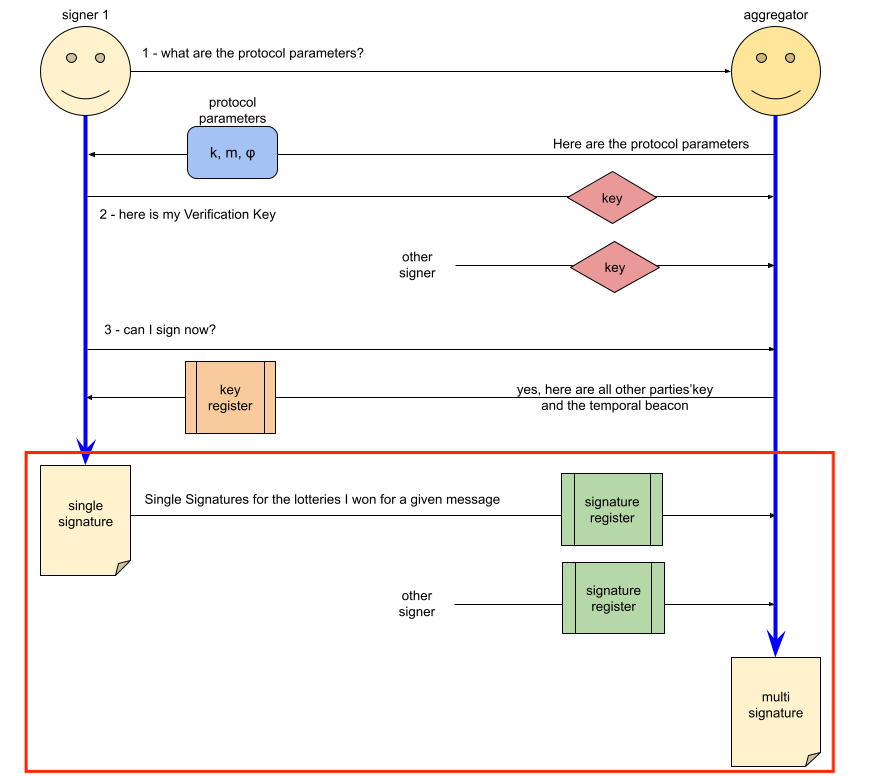
\includegraphics[width=1\linewidth]{signer-workflow-0099dc5e6cbaa76fca1cf084b510003e.png}





And we show the cost of various possible approaches:



\begin{table}[H]
    \centering
    \begin{tabular}{p{1.5cm}|p{2cm}|p{2cm}|p{2cm}|p{4cm}} \hline
          & Plonk(Halo2)&Plonk(Halo2) + BLS & Plonk(Halo2) + Groth16 & Plonk(Halo2) + Groth16 + BLS\\ \hline
          CPU cost & 3255M & 4672M & 2299M & 3716M \\ \hline
         
    \end{tabular}
    \caption{Bridge Scheme Verification Cost}
    \label{tab:my_label}
\end{table}

Note that the cost is estimated over Cardano blockchain, and results are calculated by hand, which may differ from the actual situation.





\end{document}
